\section{CRIPTOGRAFÍA MODERNA}
\subsection{Generalidades}
\begin{frame}{CRIPTOGRAFÍA MODERNA}
\framesubtitle{Generalidades}
	\begin{itemize}
      \item No se intercambian el mensaje clave, doble candado.
      \item Primos grandes
      \item Eficiencia computacional
      	\begin{equation*}
      		O((\log n)^{c\log\log\log n})
      	\end{equation*}
        \begin{equation*}
        	O(e^{\sqrt{c\log n(\log\log n)^2}})
        \end{equation*}
      \item Atkin, Sundaram, Eratosthenes \vspace{0.35cm}\footnote{\bibentry{Sieve}}
	\end{itemize}
    \begin{figure}
    	\centering
        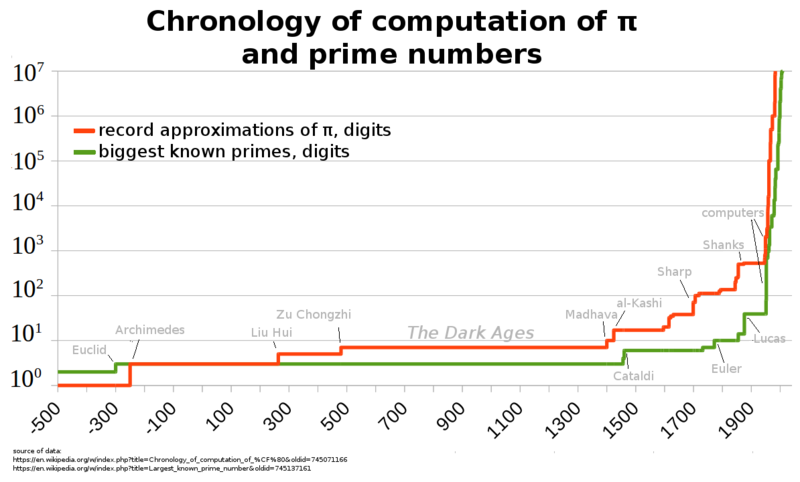
\includegraphics[scale=0.2]{chrono.png}
        \caption{Cronología de pi y los primos a través de los años\footnotemark{}.}
    \end{figure}
    \footnotetext{\bibentry{chrono}}
    \vspace{-12mm}
\end{frame}
%%%%%%%%%%%%%%%%%%%%%%%%%%%%%%%%%%%%%%%%%%%%%%%%%%%%%%%%%%%%%%%%
\subsection{Algoritmo RSA}
\begin{frame}{CRIPTOGRAFÍA MODERNA}
\framesubtitle{Algoritmo RSA}
	\begin{itemize}
	\item 1978, \textbf{R}ivest, \textbf{S}hamir \& \textbf{A}dleman.
    \item Asimétrico.
    \item Multiplicar números es sencillo, factorizarlos es difícil
	\end{itemize}
    Algoritmo: $K_U = (e,n)$, $K_R = (d,n)$
    \begin{enumerate}
    \item $p,q$ primos
    \item $n = pq$
    \item $z = (p-1)(q-1)$
    \item $e$ tal que $e$ primo, $1<e<z$ y $\texttt{GCD}(n,e) = 1$
    \item $d$ tal que $(d \cdot e) \equiv 1 \pmod{z}$
    \end{enumerate}
    Si $m$ es el mensaje original y $c$ el mensaje encriptado, entonces
    \begin{equation*}
    	c = m^e\hspace{2pt}\text{mod}\hspace{2pt} n
    \end{equation*}
    \begin{equation*}
    	m = c^d\hspace{2pt}\text{mod}\hspace{2pt} n
    \end{equation*}
\end{frame}
%%%%%%%%%%%%%%%%%%%%%%%%%%%%%%%%%
\subsection{Ejemplo RSA}
\begin{frame}{CRIPTOGRAFÍA MODERNA}
	\framesubtitle{Ejemplo RSA}
    \begin{itemize}
    \item $p=61$
    \item $q=53$
    \item $n=pq=3233$
    \item $z=(p-1)(q-1)$
    \item $e = 17$
    \item $d = 2753$
    \end{itemize}
    Tenemos $R_U = (e,n)=(17,3233)$, $R_K = (d,n) = (2753,3233)$
    Si tenemos $m = 123$, entonces
    \begin{equation*}
    	c = (123)^{17}\hspace{2pt}\text{mod}\hspace{2pt} 3233 = 855
  	\end{equation*}
    Y si se quiere descifrar,
    \begin{equation*}
    	m = (855)^{2753}\hspace{2pt}\text{mod}\hspace{2pt} 3233 = 123
    \end{equation*}
\end{frame}
